\chapter{Architektura systemu\: Backend}

\section{Stack technologiczny}
\par Warstwa \gls{Backend}owa systemu, została zaimplementowana w języku Python w połączeniu z frameworkiem \gls{FastAPI}. 
\par Wybór takiego rozwiązania został podyktowany przede wszystkim: wysoką wydajnością oraz natywnym wsparciem dla operacji asynchronicznych, co jest kluczowe w systemach zarządzania dużymi zasobami. 
\par Framework \gls{FastAPI} zapewnia również automatyczną walidację danych wejściowych we współpracy z biblioteką \gls{Pydantic}, co pozwala na minimalizację błędów w czasie działania aplikacji oraz na automatyczną generację dokumentacji \gls{API} w standardzie \gls{OpenAPI}.
\par Istotnym aspektem wyboru była także łatwa integracja z systemami bazodanowymi poprzez użycie systemu mapowania obiektowo-relacyjnego (\gls{ORM}), dostarczonego przez bibliotekę \gls{SQL Alchemy} 2.0. W połączeniu z bazą \gls{PostgreSQL} co umożliwiło bezpieczne i transakcyjne zarządzanie zasobami zapewniając integralność danych.
\par Kolejnym istotnym czynnikiem była łatwość integracji z zewnętrznymi narzędziami i bibliotekami. Wykorzystany stack technologiczny pozwolił na sprawną implementację komunikacji z systemami monitoringu (\gls{Prometheus}, \gls{Grafana}) oraz narzędziami do automatyzacji konfiguracji (\gls{Ansible}) służącymi do orkiestracji zasobów.
\par Architekturę \gls{Backend}u wzbogacono o mechanizm \gls{Redis} służący do zarządzania rozproszonymi blokadami zasobów, co jest kluczowe w przypadku środowisk wielodostępnych, gdzie jednoczesna modyfikacja zasobów przez wiele użytkowników może prowadzić do niespójności lub błędów \gls{race condition}.

\section{Architektura i wzorce projektowe}
\par Warstwa backendowa została oparta na architekturze wielowarstwowej, której celem jest odseparowanie odpowiedzialności pomiędzy osobnymi komponentami. Takie rodzaj architektury ułatwia potencjalnie skalowanie systemu w przyszłości.

\subsection{Warstwa interfejsu}
\par Warstwa odpowiedzialna za obsługę protokołu HTTP, routing, walidację schematów, wstrzykiwanie zależności odpowiedzialnych za autoryzacją i inicjalizację kontekstu użytkownika. 
\par Zaprojektowana w architekturze REST, mapując następujące operacje odpowiednio:
\begin{itemize}
    \item GET - pobieranie informacji o zasobach z bazy danych
    \item POST - wprowadzenie nowych obiektów do bazy danych
    \item PATCH/PUT - aktualizacja istniejących już obiektów w bazie danych
    \item DELETE - usuwanie istniejących obiektów w bazie danych
\end{itemize}
\begin{figure}[H]
    \centering
    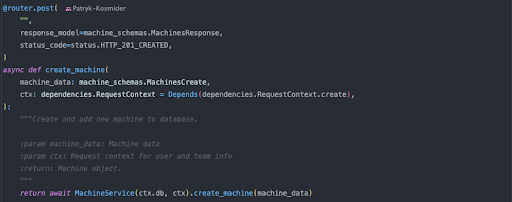
\includegraphics[width=\textwidth]{images/backend_obsluga_http.png}
    \caption{Obsługa zapytań HTTP w module machines, odpowiadająca za stworzenie nowego obiektu}
    \label{img:backend_obsluga_http}
\end{figure}

\subsection{Warstwa serwisowa}
\par Warstwa odpowiedzialna za przetwarzanie żądań dostarczonych przez użytkowników aplikacji, zgodnie z regułami biznesowymi które zostały w niej zdefiniowane. Łączy w sobie funkcjonalności wielu modułów, odpowiada za integralność i walidację biznesową, zarządza stanem i synchronizacją. Jest odizolowana od bazy danych, a także protokołu HTTP.
\begin{figure}[H]
    \centering
    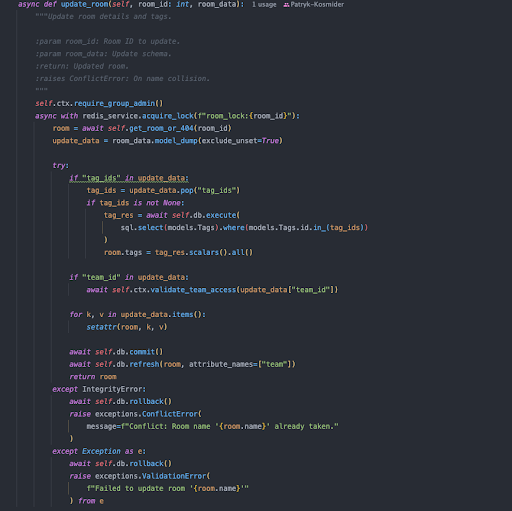
\includegraphics[width=\textwidth]{images/backend_room_service.png}
    \caption{Logika biznesowa klasy RoomService, odpowiadająca za aktualizację wartości obiektu Room}
    \label{img:backend_room_service}
\end{figure}

\subsection{Warstwa egzekutorów}
\par Specjalna warstwa abstrakcji, dedykowana do współpracy z zewnętrznymi rozwiązaniami(\gls{Ansible}, \gls{Prometheus}). Pełni rolę interfejsu pomiędzy logiką biznesową a infrastukturą zewnętrzna. W odróżnieniu od poprzednich warstw, egzekutorzy zarządzają pełnym cyklem życia wyżej wymienionych narzędzi. Dodatkowo są odpowiedzialni za hermetyzację logiki komunikacyjnej, zarządzanie stanem konfiguracyjnym, i prowadzenie autonomicznych procesów w tle.
\begin{figure}[H]
    \centering
    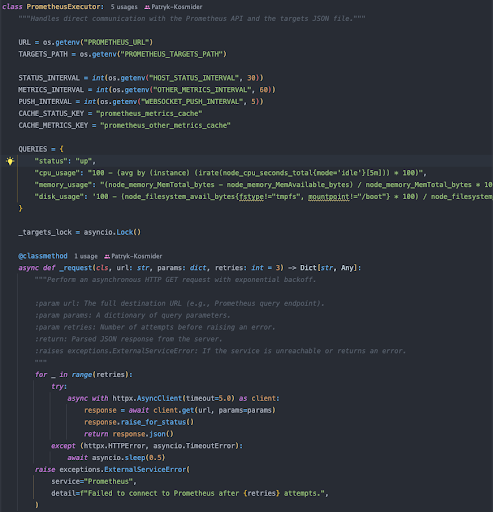
\includegraphics[width=\textwidth]{images/backend_prometheus_egzecutor.png}
    \caption{Początek klasy PrometheusExecutor, zarządzajacej komunikacją z Prometheus}
    \label{img:backend_prometheus_egzecutor}
\end{figure}
\begin{figure}[H]
    \centering
    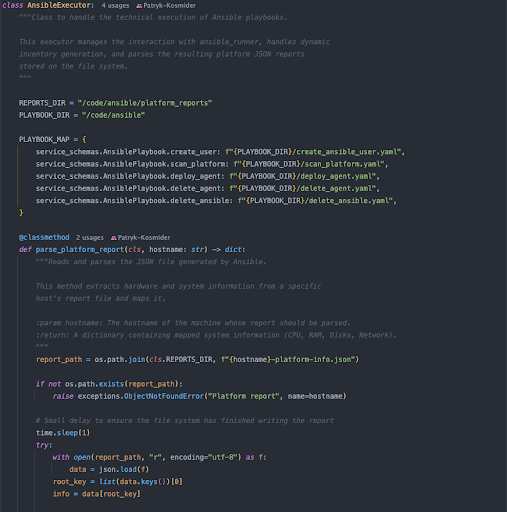
\includegraphics[width=\textwidth]{images/backend_ansible_egzecutor.png}
    \caption{Początek klasy AnsibleExecutor, zarządzającej komunikacją i egzekucją funkcjonalności Ansible}
    \label{img:backend_ansible_egzecutor}
\end{figure}

\subsection{Warstwa dostępu do danych}
\par Warstwa działająca jako pomost pomiędzy modelem obiektowym, a relacyjną bazą danych. Zawiera ona wyłącznie surowe zapytania SQL, zbudowane za pomocą \gls{ORM}. Operuje bezpośrednio na sesji bazy danych, a jej jedynym zadaniem jest wysłanie zapytania i odesłanie odpowiedzi do wyższych warstw.
\begin{figure}[H]
    \centering
    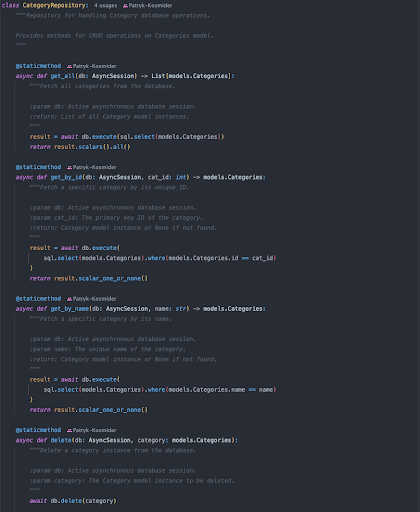
\includegraphics[width=\textwidth]{images/backend_category_repository.png}
    \caption{Repozytorium CategoryRepository, którego jedynym zadaniem jest komunikacja z bazą danych}
    \label{img:backend_category_repository}
\end{figure}

\section{Wzorce projektowe}
\par W procesie tworzenia wykorzystano następujące wzorce projektowe, by zapewnić przejrzystość i modularność kodu.
\subsection{Wstrzykiwanie zależności}
Wzorzec ten wywodzi się z fundamentalnego działania frameworka \gls{FastAPI}. Polega na przekazywaniu wymaganych komponentów do funkcji lub klas z zewnątrz zamiast tworzenia ich wewnątrz struktur. W systemie \gls{Labbyn} wzorzec ten został wykorzystany do zarządzania sesjami połączeń do bazy danych oraz mechanizmem RequestContext (Szczegółowa implementacja mechanizmu kontekstu została opisana w podrozdziale 5.3.5), zawierającym tożsamość użytkownika oraz jego uprawnienia i role. Wzorzec jest stosowano w każdym istniejącym endpoincie aplikacji. Dzięki takiemu rozwiązaniu każdy z nich otrzymuje gotowy obiekt, unikając tworzenia połączeń wewnątrz swojego ciała, co jeszcze bardziej zwiększa jego niezależność od pozostałych modułów systemu.
\begin{figure}[H]
    \centering
    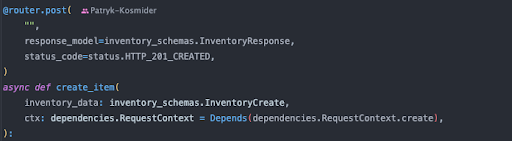
\includegraphics[width=\textwidth]{images/backend_inventory_injection.png}
    \caption{Endpoint służący do tworzenia nowego przedmiotu w inwentarzu ze wstrzyknięciem mechanizmu kontekstu}
    \label{img:backend_inventory_injection}
\end{figure}

\subsection{Singleton}
\par Wzorzec gwarantujący, że dana klasa posiada tylko jedną instancję przez cały cykl życia aplikacji oraz globalny punkt dostępu. W systemie \gls{Labbyn} wzorzec ten jest wykorzystywany do tworzenia silnika bazodanowego poprzez mechanizm cachowania modułów. Obiekt silnika jest globalny wewnątrz modułu bazy danych, przy pierwszym wywołaniu silnik bazodanowy jest inicjalizowany raz, a każda próba dostępu do niego, zawsze zwraca tą samą instancję.
\begin{figure}[H]
    \centering
    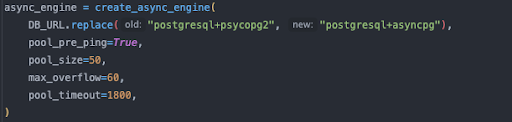
\includegraphics[width=\textwidth]{images/backend_singleton.png}
    \caption{Funkcja create\_async\_engine z pliku database.py, tworzy globalnie dostępny silnik bazodanowy}
    \label{img:backend_singleton}
\end{figure}
\par Kolejnym przykładem zastosowanego wzorca jest menadżer pamięci podręcznej \gls{Redis}. Klasa RedisClientManager przechowuje instancję klienta w atrybucie, a każda próba dosięgnięcia go sprawdza najpierw czy instancja już istnieje oraz czy jest powiązana z aktualnie działająca pętla zdarzeń zanim zostanie utworzona nowa.
\begin{figure}[H]
    \centering
    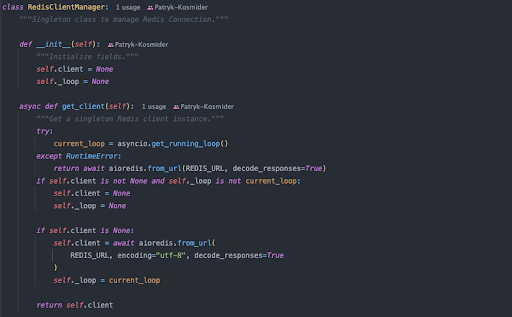
\includegraphics[width=\textwidth]{images/backend_redis_client_manager.png}
    \caption{Klasa RedisClientManager, tworzy globalnie dostępna pojedynczą instancję do komunikacji z pamięcią podręczna.}
    \label{img:backend_redis_client_manager}
\end{figure}
\subsection{Data Transfer Object}
\par Wzorzec służący do przesyłania danych między poszczególnymi elementami aplikacji, w sposób który nie ujawnia szczegółów implementacji modeli bazodanowych. W systemie \gls{Labbyn} wzorzec ten jest wprowadzony dzięki wykorzystaniu biblioteki \gls{Pydantic}. Schematy DTO definiują to, co dokładnie widzi użytkownik pozwalając wykluczać poszczególne wrażliwe elementy bazy danych, takich jak np. hasła lub ograniczać potrzebne pola, jeśli operacja nie wymaga ich wszystkich.
\begin{figure}[H]
    \centering
    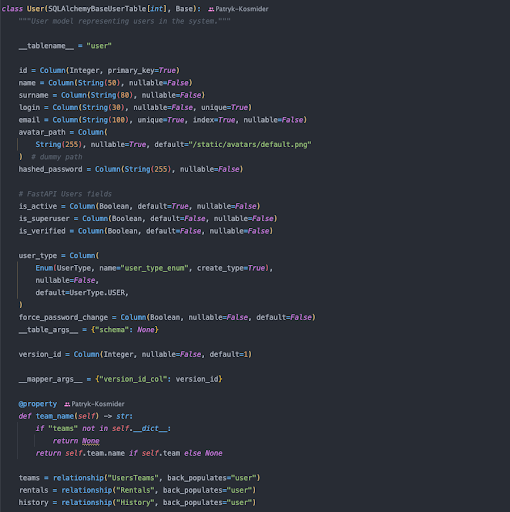
\includegraphics[width=\textwidth]{images/backend_user_model.png}
    \caption{Klasa modelująca tabele User z bazy danych do kodu}
    \label{img:backend_user_model}
\end{figure}
\begin{figure}[H]
    \centering
    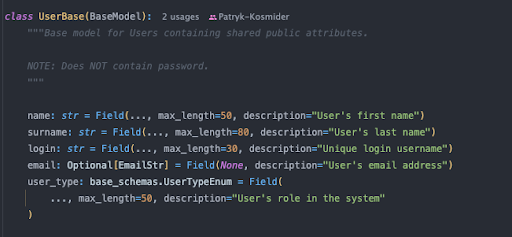
\includegraphics[width=\textwidth]{images/backend_user_dto.png}
    \caption{Schemat DTO, służący jako podstawowy schemat dla operacji związanych z użytkownikiem, powstały poprzez wykluczenie niepotrzebnych pól.}
    \label{img:backend_user_dto}
\end{figure}

\subsection{Observator}
\par Wzorzec który służy do informowania obiektów o różnych, dowolnych zdarzeniach zachodzących w obiektach, które są przez niego obserwowane. W systemie \gls{Labbyn} wzorzec ten został wykorzystany w systemie audytu. Obiektem obserwowanym jest sesja bazy danych, podczas której “obserwatorzy” rejestrują zmiany wprowadzone do określonych tabel (Machines, Inventory, Rooms, Users, Categories), i zapisują je automatycznie w tabeli History, przeznaczonej na składowanie logów (Szczegółowa implementacja mechanizmu logowania została opisana w podrozdziale 5.3.6). Dzięki takiemu zastosowaniu system \gls{Labbyn} posiada automatyczny system logowania z możliwościa łatwej manipulacji, np. poszerzeniu tabel które nas interesują.
\begin{figure}[H]
    \centering
    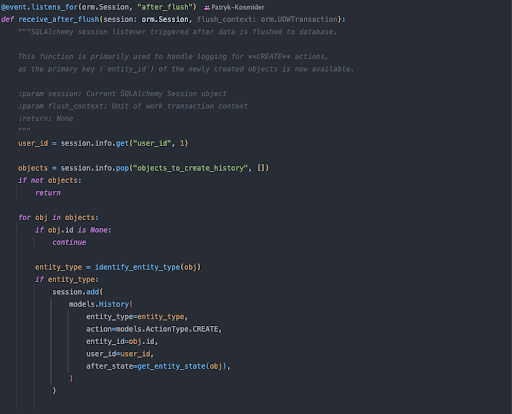
\includegraphics[width=\textwidth]{images/backend_observator.png}
    \caption{Obserwator rejestrujący zmiany dotyczące tworzenia nowych obiektów}
    \label{img:backend_observator}
\end{figure}

\section{Konfiguracja i środowisko}
\par Konfiguracja systemu \gls{Labbyn} jest podzielona na statyczne zarządzanie zmiennymi środowiskowymi obsłużonych za pomocą plików rozszerzeniem .env. Klucze dostępowe, hasła do bazy danych lub porty i adresy usług są przechowywane w plikach środowiskowych, np. api.env. Pozwala to na scentralizowane konfigurowanie środowiska, jeśli aplikacja ma zostać uruchomiona na innych portach niż domyślne, wystarczy nadpisać konkretną wartość.
\begin{figure}[H]
    \centering
    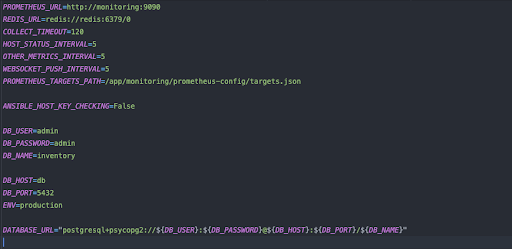
\includegraphics[width=\textwidth]{images/backend_api_env.png}
    \caption{Przykładowy plik api.env, konfigurujący parametry startowe aplikacji i zmienne globalne}
    \label{img:backend_api_env}
\end{figure}
\par W aplikacji również znajduję się mechanizm zarządzania cyklem życia, który również odpowiada za przygotowanie jej infrastruktury do pracy oraz zarządza zasobami, uruchamiany na samym starcie.
\par Podczas startu, system automatycznie tworzy potrzebną podstawową strukturę, auto inicjalizacja domyślnego admina i auto inicjalizacja pierwszego laboratorium. Serwer weryfikuje również istnienie katalogów na zasoby statyczne takie jak folder z avatarem użytkownika. Mechanizm również inicjuje procesy działające w tle służącę do monitorowania infrastruktury poprzez moduł \gls{Prometheus}, a jego prostota pozwala na rozbudowę o kolejne dodatkowe procesy.
\begin{figure}[H]
    \centering
    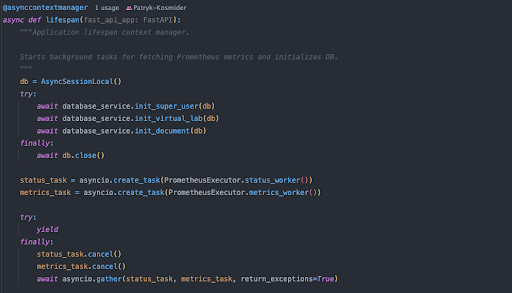
\includegraphics[width=\textwidth]{images/backend_app_lifecycle.png}
    \caption{Menedżer kontekstu inicjalizujący życie aplikacji}
    \label{img:backend_app_lifecycle}
\end{figure}
\par Kolejnym etapem środowiska jest konfiguracja \gls{CORS}, aby ograniczyć dostęp do \gls{API} wyłącznie do zaufanych źródeł, by zapobiec nieautoryzowanym żądaniom, oraz klasa StaticFiles, służąca do wystawienia katalogu pod konkretnym adresem (/static/avatars), pod którym przechowywane będą grafiki służące jako awatary użytkowników.
\begin{figure}[H]
    \centering
    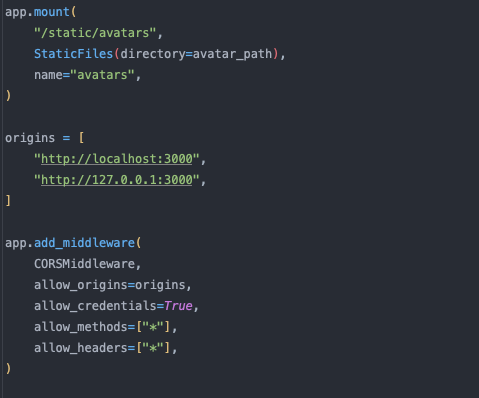
\includegraphics[width=\textwidth]{images/backend_cors.png}
    \caption{Kod inicjalizujący CORS oraz montowanie folderu dla plików statycznych}
    \label{img:backend_cors}
\end{figure}
\par Ostatnim etapem jest podłączenie routerów. Wszystkie logiczne moduły takie jak machine, rack lub tags, posiadają własne instancje klasy \gls{Router}. Wszystkie wymienione zostają podłączone do głównego cyklu życia aplikacji, co pozwala też na bardzo proste podłączenie nowych endpointów lub rezygnację z konkretnych funkcjonalności.
\begin{figure}[H]
    \centering
    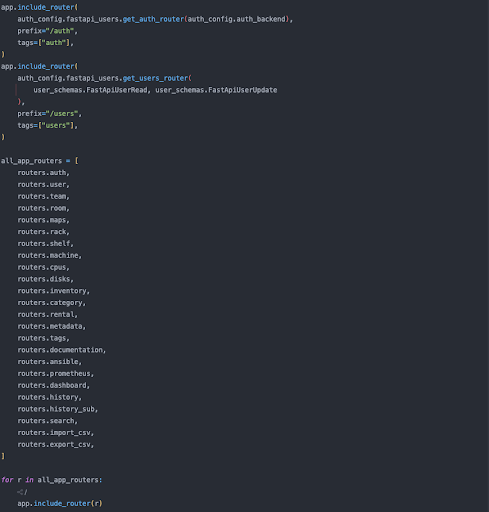
\includegraphics[width=\textwidth]{images/backedn_routers.png}
    \caption{Kod podłączający poszczególne mniejsze routery, by stworzyć pełen interfejs API}
    \label{img:backedn_routers}
\end{figure}
\par Całość znajduję się w pliku głównym main.py, co pozwala również na szybkie i proste dostosowanie aplikacji pod konkretne działanie, przez wprowadzenie minimalnych zmian.

\section{Modele danych}
\par W systemie \gls{Labbyn} warstwa danych została zrealizowana za pomocą mapowania obiektowo-relacyjnego, z wykorzystaniem biblioteki \gls{SQL Alchemy}. Pozwala to na definiowanie encji jako klas, zarządzanie typami oraz relacjami pomiędzy tabelami.
\par Wszystkie klasy modeli dziedziczą po wspólnej klasie bazowej, dzięki temu system automatycznie rejestruje tabele i ich powiązania. Każda kolumna w tabelach jest ściśle opisana poprzez parametry określające typ, relacje, i dodatkowe punkty takie jak np. możliwość pozostania pustą lub reguły usunięcia.
\par Do określenia relacji zastosowany został mechanizm relationship, który pozwala na dociąganie powiązanych ze sobą obiektów w całości, np. wyciągnięcie maszyn przypisanych do konkretnej szafy rackowej, bez potrzeby budowania skomplikowanych zapytań.
\par Dodatkowo część modeli jest wyposażona w \gls{atrybuty obliczalne}, za pomocą dekoratora @property, który pozwala na tworzenie wirtualnych pól. Oznacza to że model nie musi posiadać konkretnego pola w swojej definicji, a my możemy je dynamicznie wyciągnąć jeśli wynika ono z jego relacji z innym modelem.
\par Podstawowe encje, takie jak Machines, Rack lub Inventory, tworzące największą podstawę systemu, zostały wzbogacone o pole version\_id, służące do wprowadzenia blokady optymistycznej.
\begin{figure}[H]
    \centering
    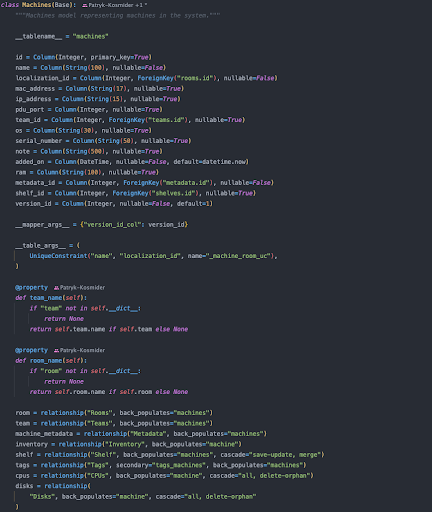
\includegraphics[width=\textwidth]{images/backend_machine.png}
    \caption{Model bazodanowy reprezentujący obiekt Machine wraz z użyciem blokady optymistycznej i atrybutów obliczalnych}
    \label{img:backend_machine}
\end{figure}
\par W celu wprowadzania zmian w strukturze bazy danych, zastosowano narzędzie Alembic. Każda zmiana w modelach jest rejestrowana jako osobny skrypt migracyjny. Dzięki takiemu rozwiązaniu jesteśmy w stanie odtworzyć strukturę bazy danych na dowolnym etapie. 
\par Narzędzie Alembic potrafi również automatycznie wykrywać różnice pomiędzy modelami w kodzie a bazą danych, generując gotowe skrypty SQL i wprowadzać je na bieżąco, by stan modeli zgadzał się z faktycznym stanem znajdującym się w bazie danych.
\par Dostarczany przez nie mechanizm migracji, pozwala na łatwe cofnięcie zmian w przypadku wykrycia błędów, by nie powodować przestojów w działaniu systemu. Każda zmiana struktury modeli, jest automatycznie rejestrowana jako rewizja, nowsza od poprzedniej, tworząc również łańcuch historii zmian.
\begin{figure}[H]
    \centering
    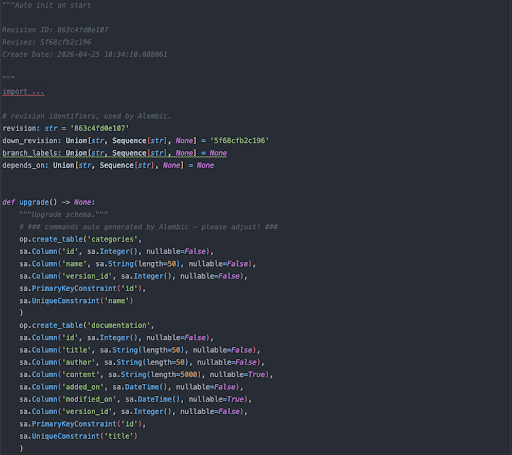
\includegraphics[width=\textwidth]{images/backend_migration_script.png}
    \caption{Przykładowy wygenerowany automatycznie w przypadku wprowadzenia zmian do modeli, skrypt migracyjny.}
    \label{img:backend_migration_script}
\end{figure}

\section{Autentykacja}
\par W warstwie autentykacji, skorzystano z rozwiązania dostarczonego przez bibliotekę \gls{FastAPI} Users, która została zintegrowana ze strategią bazodanową.
\par Zastosowano mechanizm BearerTransport, po poprawnym zalogowaniu się użytkownik otrzymuje unikatowy token przesyłany w nagłówku HTTP. Token ten zostaje zapisany do rekordu w dedykowanej tabeli access\_tokens. W przeciwieństwie do standardowego rozwiązania za pomocą tokenów JWT, ta strategia pozwala na natychmiastowe przerwanie sesji w przypadku wykrycia nieprawidłowości, lub usunięcia konta użytkownika, co pozwala na jeszcze większe podniesienie standardów bezpieczeństwa.
\begin{figure}[H]
    \centering
    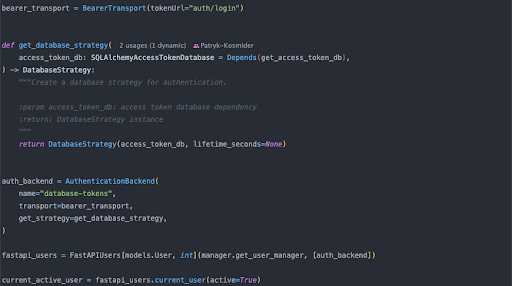
\includegraphics[width=\textwidth]{images/backend_auth_strategy.png}
    \caption{Konfiguracja autentykacji i strategii przechowywania tokenów}
    \label{img:backend_auth_strategy}
\end{figure}
\par By zarządzać procesem logowania, skorzystano z gotowego mechanizmu dostarczonego przez \gls{FastAPI} Users, który został poszerzony ręcznie, specjalnie w celu dostosowania go do systemu \gls{Labbyn}. 
\par Standardowe mechanizmy logowanie zostały nadpisane by umożliwić identyfikację użytkowników poprzez unikalny login, co jest bardziej praktyczne w rozwiązaniach wewnętrznych. Dzięki temu system w pierwszej kolejności weryfikuję tożsamość na podstawie loginu, następnie korzysta z wbudowanej funkcji do procesu weryfikacji hasła, które jest zabezpieczone za pomocą BCrypt. Każde hasło przed zapisem do bazy jest poddawane procesowi hashowania.
\begin{figure}[H]
    \centering
    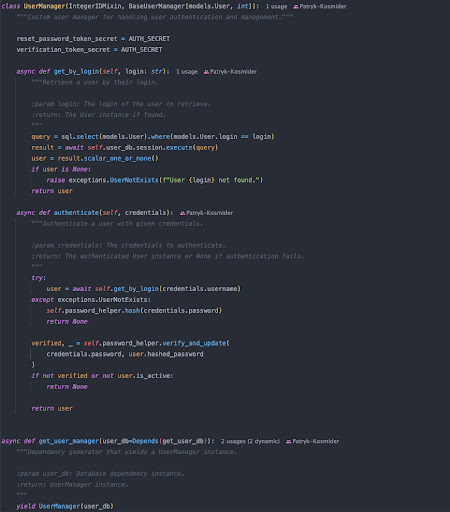
\includegraphics[width=\textwidth]{images/backend_user_manager.png}
    \caption{Klasa UserManager, poszerzona o możliwość logowania się za pomocą loginu}
    \label{img:backend_user_manager}
\end{figure}
\par W celu zapewnienia maksymalnej kontroli nad dostępem do infrastruktury, wdrożono własny system zarządzania hasłami. W przypadku inicjalizacji konta, system generuje jednorazowe hasło startowe, który jest przekazywane przez administratora użytkownikowi. Przy pierwszym logowaniu system zmusza użytkownika do zdefiniowania własnego hasła. W przypadku resetu hasła, administrator ustawia hasło tymczasowe i aktywuję flagę resetu. Następnie analogicznie przekazuje nowo wygenerowane jednorazowe hasło użytkownikowi, który jest zmuszony po zalogowaniu zmienić je na własne.
\begin{figure}[H]
    \centering
    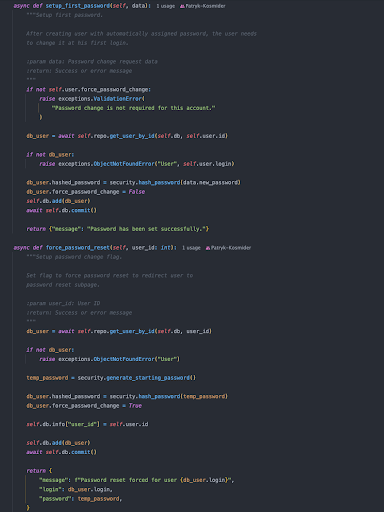
\includegraphics[width=\textwidth]{images/backend_auth_service.png}
    \caption{Klasa AuthService, serwis posiadający metody do resetowania hasła i obsługi pierwszego zalogowania}
    \label{img:backend_auth_service}
\end{figure}


